\chapter*{Prefaci} \addcontentsline{toc}{chapter}{Prefaci}

   Voldria dir en primer lloc que no he intentat escriure un tractat complet
   d'electrotècnia, d'electrònica o de sistemes elèctrics de potència, sinó que més aviat
   he volgut
   fer una recopilació de qüestions teòriques i pràctiques relacionades amb els camps mencionats
   anteriorment.

   Les fonts d'informació utilitzades en la realització d'aquest llibre són molt diverses,
   i inclouen llibres sobre les diferents matèries, articles de revistes o d'Internet,
   apunts de classe d'assignatures impartides a l'ETSEIB,\index{ETSEIB} i d'altres.

   Pel que fa al llibre en si mateix, ha estat escrit utilitzant el sistema de composició de
   textos \LaTeX,\index{LaTex@\LaTeX} el qual
   permet integrar molt fàcilment text, fórmules i gràfics, obtenint un resultat de
   gran qualitat. S'han utilitzat diversos paquets d'ampliació, com ara
   l'\AmS-\LaTeX,\index{AmSLaTex@\AmS-\LaTeX}
   per tal de millorar la presentació de certes parts del
   llibre, com per exemple les taules, les capçaleres o les fórmules matemàtiques. S'ha utilitzat la distribució MiK\TeX, que ofereix una implementació lliure de \LaTeX , accessible a l'adreça: \href{http://www.miktex.org/}{www.miktex.org}.

   Aquest llibre està pensat per  ser utilitzat tant de forma directa en la pantalla d'un
   ordinador com en paper després d'haver-lo imprès; per tal d'estalviar paper, el text
   té un format pensat per  ser imprès en paper DIN-A4,\index{DIN-A4} a dues cares.

    El contingut del llibre és molt divers, i va des de temes força teòrics fins a
    d'altres bastant més pràctics. He procurat donar exemples de tots els conceptes
    que s'hi expliquen, excepció feta dels molt elementals, perquè crec que és important
     no quedar-se només amb la teoria de  la resolució d'un problema determinat, sinó que
     és molt útil veure exemples resolts pas a pas. En alguns exemples s'utilitzen programes de càlcul matemàtic o calculadores científiques per tal de resoldre els exemples més fàcilment. Una part  del llibre està dedicada al llenguatge de programació Python, en el seu vessant científic i tècnic, i al seu ús  per resoldre molts dels exemples del llibre.

	El llibre està dividit en sis parts amb el següent contingut:
	\begin{itemize}
		\item Part I --- Electrotècnia. 
		\begin{itemize}
			\item El capítol 1 comença presentant les equacions bàsiques que lliguen tensions, corrents i potències en els components elementals de l'electrotècnia --- resistències, condensadors, inductàncies, etc. --- tant en el domini freqüencial com en el domini operacional. A continuació s'expliquen els teoremes de Thévenin-Norton, de Millman i de la superposició. Tot seguit es donen equacions i taules per calcular els valors mitjans i eficaços de diverses formes d'ona, així com la definició de diversos factors de forma, d'arrissada, etc. S'expliquen a continuació els conceptes de potència instantània i els de potència complexa monofàsica i trifàsica. L'apartat següent es dedica  als circuits R-L-C de corrent continu i altern, i per acabar s'explica el mètode de les malles per a la resolució de xarxes elèctriques.
			\item El capítol 2 està dedicat a diversos càlculs bàsics i freqüents de l'electrotècnia. S'explica primer el sistema de càlcul en per unitat. Es tracten a continuació els circuits  divisors de tensió i corrent,  les transformacions estrella-triangle d'impedàncies, i la resolució de problemes on es coneix la potència consumida per una càrrega, però no la seva impedància. En el següent apartat es donen equacions pel càlcul simplificat del corrent de curtcircuit en el secundari de transformadors, i per acabar es tracten  qüestions relatives a les  escales gràfiques logarítmiques.
			\item El capítol 3 està dedicat a les components simètriques. Es donen les equacions d'aquest mètode de càlcul, es presenten les components directa, inversa i homopolar, i la seva relació amb el corrent de neutre. A continuació es tracta el càlcul de la potència elèctrica a partir de les components simètriques de tensions i corrents, i per acabar es presenten diversos programes de la calculadora \textsf{HP Prime} relacionats amb aquestes qüestions.
			\item El capítol 4 està dedicat a l'aplicació de les sèries de Fourier a la resolució de problemes electrotècnics. Es comença per definir la sèrie de Fourier d'una funció periòdica i es donen les equacions de càlcul dels seus paràmetres; s'expliquen  les simplificacions que són d'aplicació a certes funcions --- parells, senars i amb simetria de semiona --- i es defineix la condició de Dirichlet en els punts de discontinuïtat. Es donen a continuació les fórmules per calcular el valor mitjà i eficaç, i diversos paràmetres característics. Seguidament es presenta una taula amb la sèrie de Fourier de diverses formes d'ona i algunes propietats útils per utilitzar aquesta taula. S'explica finalment com calcular la potència a partir de les sèries de Fourier de tensions i corrents, i s'aplica de forma pràctica les sèries de Fourier a l'anàlisi de circuits elèctrics.
			\item El capítol 5  està dedicat a l'aplicació de la transformada de Laplace a la resolució de problemes electrotècnics. Es comença per definir la transformada de Laplace i la transformada inversa de Laplace i es donen les equacions de càlcul; es defineix també la funció graó  unitari i la funció impuls. Es defineixen a continuació diverses propietats de la transformada de Laplace --- linealitat, canvi d'escala, translació, etc. Seguidament es presenta una taula amb la transformada de Laplace de diverses funcions i de diverses formes d'ona. Finalment s'aplica de forma pràctica la transformada de Laplace a l'anàlisi de circuits elèctrics, inclosa una explicació detallada de les fraccions parcials.
		\end{itemize}
		\item Part II --- Equips i Components Elèctrics. 
		\begin{itemize}
			\item El capítol 6 presenta  la codificació en colors de les resistències, segons la norma CEI 60062 \textit{Marking codes for resistors and capacitors}. També dona els valors estandarditzats de les resistències, segons la norma CEI 60063 \textit{Preferred number series for resistors and capacitors}.
			\item El capítol 7 està dedicat als cables elèctrics. Es donen les fórmules de càlcul de la caiguda de tensió i de la capacitat tèrmica en curtcircuit, s'expliquen  les unitats americanes usades per mesurar els diàmetres i les seccions dels cables --- mil, cmil, kcmil i AWG --- i es donen també les taules i fórmules necessàries per convertir-les a les  unitats mètriques equivalents --- mm i \unit{mm^2}.
			\item El capítol 8 està dedicat als transformadors de mesura i protecció, tant de tensió com de corrent. La major part del capítol està dedicat a la norma CEI 60044 \textit{Instrument transformers}, però es descriu també més breument  la norma IEEE C57.13 	\textit{	Requirements for Instrument Transformers}, i la relació entre ambdues.
			\item El capítol 9 està dedicat als transformadors de potència. S'introdueix l'esquema elèctric equivalent d'un transformador a partir dels valors reals en  ohm i a partir dels valors reduïts en per unitat, i s'obté el circuit equivalent Thévenin vist des del secundari. Es defineixen els paràmetres: rendiment,  caiguda de tensió i regulació de voltatge. Es descriuen els assajos fets a un transformador  --- en buit i en curtcircuit --- i es donen les fórmules necessàries per obtenir els paràmetres del circuit equivalent a partir dels valors dels assajos. S'explica també les característiques particulars dels transformadors trifàsics, com ara el grup horari de connexió,  els circuits elèctrics equivalents per a tensions de seqüència  homopolar i  negativa, o la connexió en paraŀlel de transformadors.
			\item El capítol 10 està dedicat als motors d'inducció trifàsics, prenent com a punt de partida el circuit elèctric equivalent del motor. En primer lloc es fa una breu introducció  a les unitats de mesura angleses utilitzades en l'àmbit dels motors, ja que hi ha molts llibres, articles tècnics i catàlegs que utilitzen aquestes unitats. Es donen a continuació una sèrie de fórmules bàsiques dels motors, incloent-hi la que permet calcular-ne els temps d'arrancada. Es presenta a continuació l'esquema elèctric equivalent d'un motor, i es desenvolupen totes les equacions que permeten trobar   corrents, tensions, parells, potències, factor de potència i rendiment. Es presenta també el circuit elèctric equivalent del motor per a tensions 
			de seqüència negativa, i es tracta el cas de motors que funcionen a potència reduïda o a tensió d'alimentació reduïda. Finalment,  es tracten qüestions relatives a la norma NEMA MG-1 \textit{Motors and Generators}. 
		\end{itemize}
		\item Part III --- Sistemes Elèctrics de Potència. 
		\begin{itemize}
			\item El capítol 11 explica el mètode dels nusos per a la resolució de xarxes elèctriques. Aquest és un mètode sistemàtic per resoldre xarxes elèctriques --- permet calcular la tensió i el corrent de totes les branques de la xarxa --- formades per fonts de tensió i de corrent, resistències, inductàncies, capacitàncies, i induccions mútues entre branques. També permet calcular el circuit Thévenin equivalent entre qualsevol parell de nusos de la xarxa.
			\item El capítol 12 tracta la resolució del problema del flux de càrregues en sistemes 	elèctrics de potència. En aquests tipus de problemes les dades no són les fonts de tensió i impedàncies de les càrregues, sinó que són les potències activa i reactiva absorbides o subministrades, i el mòdul i l'argument de la tensió, en els diversos nusos de la xarxa. En cada nus només es coneixen alguns dels quatre valors indicats, i el mètode explicat en aquest capítol permet trobar els valors restants, així com el flux de potència que circula per les branques de la xarxa. Es presenten també els models matemàtics de les línies de transmissió i dels transformadors de potència, que són necessaris per a la resolució del flux de càrregues.
			\item El capítol 13 està dedicat a  diverses normes. En concret s'explica la norma IEEE C37.2 \textit{Electrical Power System Device Function Numbers and Contact Designations}, sobre la numeració utilitzada per designar les funcions i proteccions elèctriques; la codificació IP segons la norma CEI 60529 \textit{Degrees of protection provided by enclosures (IP code)}, que codifica el grau de protecció proporcionat pels 			elements envoltants d’equips elèctrics; la codificació IK segons  la norma CEI 62262 \textit{Degrees of protection provided by enclosures for 			electrical equipment against external mechanical impacts (IK Code)}, que  codifica la resistència d’un
			element envoltant als impactes mecànics; la norma
			NEMA 250 \textit{Enclosures for Electrical Equipment (1000 Volts Maximum)}, que descriu codis similars al IP; i la norma CEI 60947-2 \textit{Low-voltage switchgear and controlgear --- Circuit-breakers}, sobre els interruptors automàtics de baixa tensió. Les dues seccions finals es dediquen al llistat de normes de la CEI \textit{Commission électrotechnique internationale} i de la IEEE \textit{Institute of Electrical and Electronics Engineers}, agrupades per àmbits d'aplicació.
		\end{itemize}
		\item Part IV --- Python. 
		\begin{itemize}
			\item El capítol 14 fa una breu introducció al llenguatge de programació Python.
			\item El capítol 15 presenta dos mòduls de Python amb classes i funcions dedicats a la resolució de problemes electrotècnics.
			\item El capítol 16 està dedicat  a la resolució dels exemples del llibre mitjançant el llenguatge de programació Python. Els exemples del llibre que estan resolts mitjançant Python tenen el símbol (\faPython) afegit al final del seu títol; aquest símbol és un enllaç que porta directament a l'apartat del capítol 16 on es resol l'exemple.
		\end{itemize}
		\item Part V --- Apèndixs. 
		\begin{itemize}
			\item L'apèndix A presenta breument l'alfabet grec, amb la grafia i el nom de cadascuna de les lletres que el formen.
			\item L'apèndix B explica el Sistema Internacional d'unitats, tal com està definit pel \textit{Bureau International des Poids et Mesures} (BIPM). S'introdueixen també algunes unitats de la norma CEI 60027 \textit{Letter symbols to be used in electrical technology}, com ara les informàtiques, les de potència elèctrica, i les relatives a màquines rotatives. Es dedica també una secció sencera a explicar les normes d'escriptura de valors numèrics acompanyats d'unitats.
			\item L'apèndix C llista els valors d'una sèrie de constants de la natura, segons la  publicació
			de l’any 2018 del \textit{Committee on Data for
			Science and Technology} (CODATA). S'explica també com es llegeixen els errors absoluts d'aquestes constants i com se n'obté l'error relatiu.
			\item L'apèndix D presenta una sèrie de relacions matemàtiques de les funcions trigonomètriques i de les funcions hiperbòliques. També es donen relacions matemàtiques dels angles i dels costats d'un triangle; això és útil en el cas de sistemes trifàsics on apareixen triangles de fasors que representen tensions.
			\item L'apèndix E està dedicat breument al càlcul numèric, i s'introdueixen algoritmes de càlcul relatius a la interpolació, la integració i la resolució d'equacions no lineals.
			\item L'apèndix F llista una sèrie de programes per a la calculadora \textsf{HP Prime} de Hewlett-Packard que són útils per resoldre problemes elèctrics. 
		\end{itemize}
		\item Part VI --- Bibliografia i  Índex Alfabètic.
	\end{itemize}
		

    Encara que he fet tots els esforços possibles per eliminar qualsevol
    mena  d'error en aquest text, és gairebé inevitable que n'hagi quedat algun,
    per tant, si algú troba algun error farà bé d'avisar-me!


   Únicament em resta dir que espero que els lectors d'aquest llibre el trobin    útil i interessant, de la mateixa manera que la seva escriptura m'ha resultat  instructiva a  mi mateix.


\hfill
\begin{minipage}[b]{35mm}
    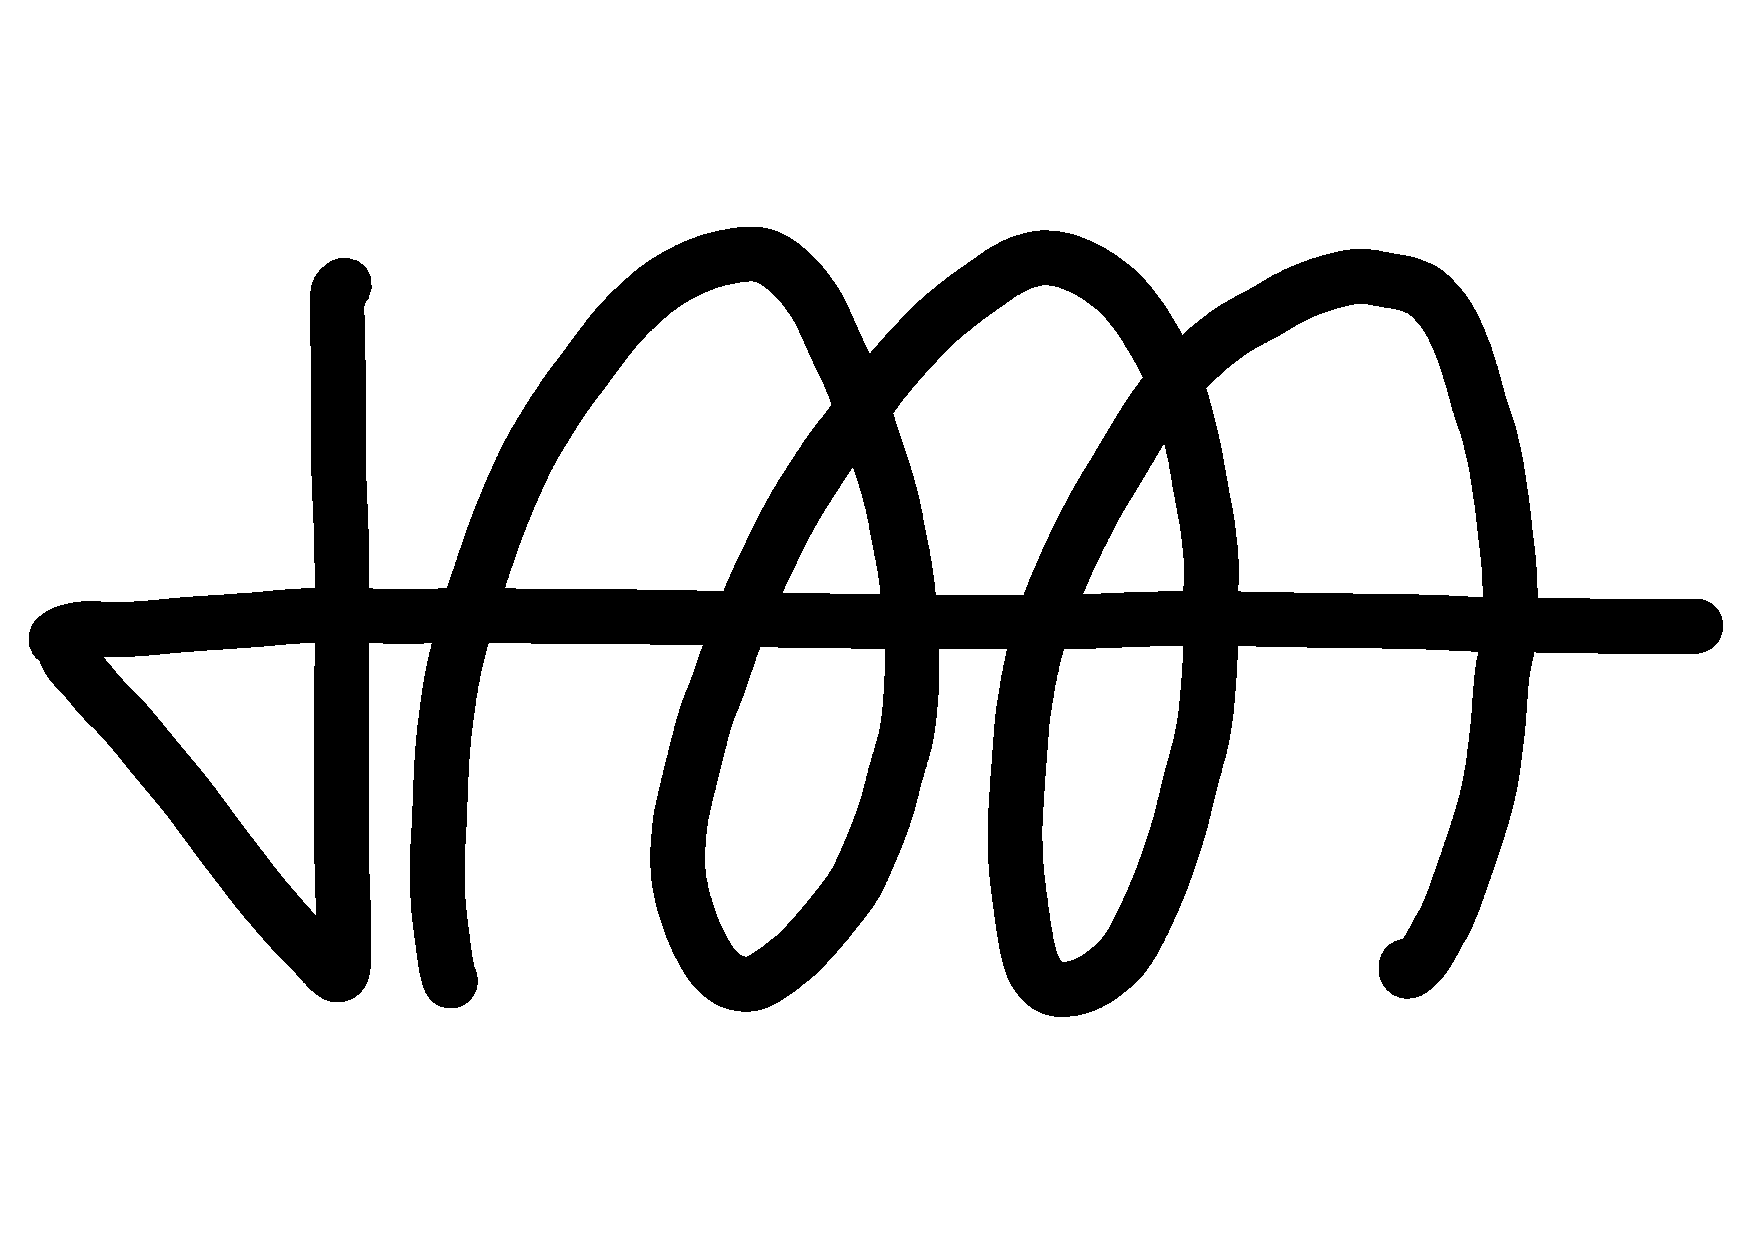
\includegraphics[scale=0.1]{Pre-firma-JMB.pdf}
\end{minipage}

{\large

    \hfill \textbf{\textsl{Josep Mollera Barriga}}

    \hfill \textbf{\textsl{29 de juliol de 2022}}

    \hfill {\small \href{mailto:jmb.qed@outlook.com}{\faEnvelope\hspace{2mm}jmb.qed@outlook.com} }

}
